\chapter{Introduction}

\section{Why Study Fractional Calculus?}
Some people may study fractional calculus because it is inherently interesting to them. Other people need more or different reasons. A few reasons include:
\begin{itemize}
  \item Fractional calculus expands the descriptive power of calculus beyond the familiar integer order derivatives and the basic concept of rate of change. This will yield more accurate descriptive equations when a system truly is fractional.
  \item Fractional calculus can expand scientific understanding when it models things that are traditionally very difficult to describe mathematically.
  \item Integer order derivatives are \emph{local} needing information only in a neighborhood of a point. As will be seen, fractional derivatives are \emph{non-local} and can describe systems with such a feature. For example, $F=ma$ right \emph{now}. How something accelerates only depends on the forces right now, not the forces at any time in the past. For systems with ``memory'' effects, or analogous non-local spatial effects, the differential equation describing it most accurately may be fractional.
\end{itemize}

It is not surprising that ``normal'' integer-order calculus works well for most engineering applications over the past few centuries. Newton, who was one of the very early developers of calculus, clearly had a strong interest in mechanics \cite{principia}. However, there are a couple topics of more recent interest in engineering for which fractional calculus may be important. One area is bioengineering, where traditional mechanics and electromagnetism do not fully describe the system and in which non-local time effects may occur. Another is very large scale systems that may be easier to consider as having an infinite number of components, rather than keeping track of every single part. Examples of each type are given in this chapter.  Finally, fractional calculus has been used as a new tool to try to match measured responses to ``generally hard to model'' system, \textit{e.g.}, systems with friction, stiction, etc. 

\section{Introductory Concepts}
Anyone reading this book should be familiar with the notion of the first, second and higher derivatives, \textit{e.g.}, for $f(t) = t^3 + 5 t^2 + 2$, 
\begin{align}
  \frac{\d f}{\d t}(t) &= 3 t^2 + 10 t \\
  \frac{\d^2 f}{\d t^2}(t) &= 6t + 10, 
  \label{eq:derivs}
\end{align}
\textit{etc.} Also we naturally think of integrals in an antiderivative sense, \textit{e.g.},
\begin{align}
  \int f(t) \d t &= \frac{1}{4} t^4 + \frac{5}{3} t^3 + 5 t^2 + c 
  \label{eq:integrals}
\end{align}
and we adopt a notation of $f^{(1)}(t)$ as the first derivative, $f^{(2)}(t)$ as the second derivative and $f^{(n)}(t)$ as the $n$th derivative as well as $f^{(-1)}(t)$ as $f$ integrated one time, $f^{(-2)}$ as $f$ integrated two times, \textit{etc.}

A mathematically curious reader may already be wondering if there are any derivatives ``in between'' the integer ones.
For example, is there a one-half derivative:
\begin{equation}
  \frac{\d^\frac{1}{2} f}{\d t^\frac{1}{2}}(t) = f^{\left(\frac{1}{2}\right)} = ?.
  \label{eq:halfderiv}
\end{equation}
There is not an immediate obvious answer to this because of the fact that the integer order derivative (as is the integral) is defined as a limit
\begin{equation}
  \frac{\d f}{\d t}(t) = \lim_{\Delta t \rightarrow 0} = \frac{f\left(t + \Delta t \right) - f\left(t\right)}{\Delta t}
  \label{eq:limdef}
\end{equation}
and that is a discrete operation. There is not a natural half way to do it.

Basically we want to generalize the notion of the derivative. In a sense, if we define something to give the, say $\alpha$ derivative where $\alpha \in \mathbb R$, \textit{i.e.}, $\alpha$ is a real number, then all we really need is that when $\alpha$ is an integer we get the usual definition of that integer order derivative. In between there may be lots of different options (there are!), but it makes sense to set some other basic requirements we want a fractional-order derivative to satisfy.

\begin{example}
  Consider $f(t) = t^2$ with the first and second derivatives $f^{(1)}(t) = 2 t$ and $f^{(2)}(t) = 2$, respectively. We should expect that the $1/2$ derivative is, in some qualitative sense, ``between'' $f(t)$ and $f^{(1)}(t)$, and that the $3/2$ derivative is ``between'' the first and second derivatives, as is illustrated in Figures~\ref{fig:fracidea1} and \ref{fig:fracidea2}.

  \begin{figure}
    \centering
    \subimport{figs/}{fracidea}
    \caption{The zeroth and first derivatives of $f(t)=t^2$, (blue and red curves). A prospective half derivative (gold).}
    \label{fig:fracidea1}
  \end{figure}

  \begin{figure}
    \centering
    \subimport{figs/}{fracidea2}
    \caption{The first and second derivatives of $f(t)=t^2$ (blue and red curves) with a prospective $3/2$ derivative (gold).}
    \label{fig:fracidea2}
  \end{figure}

  We also expect that as we vary the order of the derivative, say from $0$ to $1$, for low values of the order the result is near the zeroth derivative, and for values of the fractional order near one, it is near the first derivative. This is illustrated in Figure~\ref{fig:fracidea3}.

  \begin{figure}
    \centering
    \subimport{figs/}{fracidea3}
    \caption{The function (blue) and the first derivative (red). The $0.2$, $0.4$, $0.6$ and $0.8$th (yellow, purple, green, light blue) order derivatives ``move'' from the zeroth derivative to the first derivative.}
    \label{fig:fracidea3}
  \end{figure}
\end{example}

This example motivates our first desirable attribute of a fractional derivative.

\begin{attribute}
  For a fractional derivative, $f^{\left( \alpha \right)}(t)$, if $\alpha$ is near an integer value, we expect the $\alpha$ derivative to be near that integer derivative of $f(t)$. As $\alpha$ varies between integer values, we expect that $f^{\left( \alpha \right)}(t)$ varies in a reasonable manner between those integer values.
\end{attribute}

\section{Fractional Derivatives of some Elementary Functions}
\subsection{Sine and Cosine Functions}
As a first step into some real functions, we consider sine and cosine.

\begin{example}
  Consider $f(t) = \sin(t)$. The nice thing about sines and cosines are their relatively simple derivatives. In fact, from the pattern
  \begin{align*}
    \frac{\d}{\d t} \sin(t) &= \cos(t) \\
    \frac{\d^2}{\d t^2} \sin(t) &= -\sin(t)
  \end{align*}
  as illustrated in Figure~\ref{fig:fracidea4}, it is clear that the derivative for this function just shifts it to the left by $\pi/2$. So clearly we would expect that the $1/2$ derivative just shifts it to the left by $\pi/4$, or the $1/2$ integral shifts it right by $\pi/3$, \textit{etc}. Therefore, a reasonable guess for the half derivative would be as illustrated in Figure~\ref{fig:fracidea5}.

  \begin{figure}
    \centering
    \subimport{figs/}{fracidea4}
    \caption{First (red) and second (gold) derivative of $\sin(t)$ (blue). The arrows indicate that derivative is just shifts the curve to the left by $\pi/2$ for each derivative.}
    \label{fig:fracidea4}
  \end{figure}

  \begin{figure}
    \centering
    \subimport{figs/}{fracidea5}
  \caption{Reasonable assumption for the half derivative (red) of $\sin9t)$ (blue).}
  \label{fig:fracidea5}
\end{figure}

\end{example}

\subsection{Monomials and Polynomials}

Being able to take the fractional derivative of sine and cosine functions is nice, but we would like to do more. The next easiest class of functions is polynomials. Consider 
\begin{equation}
  f(t) = t^k
  \label{eq:poly}
\end{equation}
which is easy to differentiate a few times and figure out the pattern:
\begin{align}
  \frac{\d f}{\d t}(t) &= k t^{k-1} \\
  \frac{\d^2 f}{\d t^2}(t) &= k \left( k-1 \right) t^{k-2} \\
  \frac{\d^3 f}{\d t^3}(t) &= k \left( k-1 \right) \left( k - 2 \right) t^{k-3} \\
  \vdots &= \vdots \\
  \frac{\d^n f}{\d t^n}(t) &= \frac{k!}{\left( k - n \right)!} t^{k-n}, \qquad n \leq k.
  \label{eq:polyderivs}
\end{align}
Since we are looking to define a fractional derivative of $t^k$, we need to see what is allowed and not allowed for $n$ to take on fractional values in Equation~\ref{eq:polyderivs}. The exponent of $t$ can be a fraction (more about that later, but engineers are so used to it they may not remember where it came from). What is definitely a problem, though, is the factorial in the denominator: if $k$ is a natural number and $n$ is not an integer, then the factorial is not defined.

The factorial function is just a series of values, so it seems we can generalize the derivative of $t^k$ if we can find a curve through the factorial values. In fact, of course, it has been done and it is the gamma function defined by
\begin{equation}
  \Gamma\left(z\right) = \int_0^\infty x^{z - 1} e^{-x} \d x
  \label{eq:gamma}
\end{equation}
which is plotted for positive real values of $z$ in Figure~\ref{fig:gamma}. Clearly, for integer values
\begin{equation}
  z! = \Gamma\left( z + 1 \right).
\end{equation}

\begin{figure}
  \centering
  \subimport{figs/}{gamma}
  \caption{Plot of $\Gamma(z)$ (blue curve) and some factorials, $\left(z - 1\right)!$ (red).}
  \label{fig:gamma}
\end{figure}

So, returning to Equation~\ref{eq:polyderivs}, it seems that all we need to do to define a fractional derivative is to replace the factorial in the denominator with the gamma function shifted by one. Purely for aesthetics, we might as well use a gamma function in the numerator as well, which also then would allow for a fractional $k$. So, we have the following seemingly legitimate definition of a fractional derivative for a monomial.

\begin{definition}
  For the monomial, $t^k$, $k \in \mathbb R$, define a\footnote{This is \emph{a} fractional derivative, rather than \emph{the} fractional derivative because there are many definitions. } proposed fractional derivative 
  \begin{equation}
    \boxed{
    \frac{\d^\alpha}{\d t^\alpha} t^k = \frac{\Gamma\left( k + 1 \right)}{\Gamma \left( k + 1 - \alpha \right)} t^{k - \alpha} }
    \label{eq:monomialfrac}
  \end{equation}
  for real values of $\alpha$, \textit{i.e.}, $\alpha \in \mathbb R$.
  \label{def:monomialfracderiv}
\end{definition}

This definition was used to make the fractional derivative curves in Figures~\ref{fig:fracidea1} through
\ref{fig:fracidea3}, so in a sense it has been validated. Also, because everything we have done is linear in $t$, we can
use this definition for monomials and extend it term-by-term to polynomials. 

For fun, we will do and example with a different $k$ and also include negative values for $\alpha$ to see if integral-like ideas appear.

\begin{example}
  Consider $f(t) = t^\frac{1}{2} = \sqrt{t}$. Various fractional order derivatives and integrals computed using Equation~\ref{eq:monomialfrac} in Definition~\ref{def:monomialfracderiv} are illustrated in Figure~\ref{fig:monex}.

  \begin{figure}
    \centering
    \subimport{figs/}{monex}
    \caption{Various fractional derivatives using Definition~\ref{def:monomialfracderiv} for $f(t) = \sqrt{t}$. The thick blue curve is the function, or zeroth derivative. The red curve is the $\alpha = -1$ derivative, which does correspond to the integral. The gold curve is the $\alpha = -1/2$ derivative, or the $1/2$ integral. The green and light blue curves are the $1/2$ and first derivatives, respectively.}
    \label{fig:monex}
  \end{figure}
\end{example}


\subsection{Exponentials}
Since
\begin{equation*}
  \frac{\d^n}{\d t^n}e^t = e^t
\end{equation*}
we would like it to also hold for when $n$ is not an integer.  Similarly, 
\begin{equation*}
  \frac{\d^n}{\d t^n} e^{\alpha t} = \alpha^n e^{\alpha t}
\end{equation*}
we can require that the same, or something close to this, be true when $n$ is not an integer.

At this point we can compute things we consider to be fractional derivatives and integrals of sines and cosines, monomials, by extension from monomials, polynomials if we do them term-by-term and exponentials.  Before we generalize further, in order to develop a very important property of the fractional derivatives, we need to go a long way back and consider fractional exponents.



\section{The Law of Indices}

Engineers deal with fractional and negative exponents so often that it is easy to lose track of why they actually make sense. The exponent is defined for natural numbers (integers greater than zero) as the number of times the base is multiplied by itself, \textit{i.e.},
\begin{equation}
  t^n = \underbrace{t \times t \times t \cdots t \times t}_{\mbox{$n$ times}}.
  \label{eq:power}
\end{equation}
An obvious property of this is that for two natural number exponents
\begin{align}
  \left(t^n\right) \times \left( t^m \right) &=  \left( \underbrace{t \times t \times t \cdots t \times t}_{\mbox{$n$ times}}
  \right) \times \left( \underbrace{t \times t \times t \cdots t \times t}_{\mbox{$m$ times}}
  \right) \\
  &= 
  \underbrace{t \times t \times t \cdots t \times t}_{\mbox{$n + m$ times}} \\
  &= t^{n + m}
  \label{eq:indices}
\end{align}
which also immediately leads to
\begin{equation}
  \left( t^n \right)^p = t^{n \times p}.
  \label{eq:indices2}
\end{equation}
This notion of adding indices can be used to \emph{define} negative and fractional exponents by requiring that Equations~\ref{eq:indices} and \ref{eq:indices2} hold for all rational values as well (negative values, zero and fractional values). 

For negatives values, consider $n$ and $m$ to be positive integers with $n > m$, and if we require that $\left( t^n \right) \times \left( t^{-m} \right) = t^{n-m}$, then the only way for the $-m$ to take away powers is for it to mean division, or in too much detail
\begin{equation}
  t^n \times t^{-m} = \frac{\overbrace{t \times t \times t \cdots t \times t}^{\mbox{$n$ times}}}{\underbrace{t \times t \cdots t \times t}_{\mbox{$m$ times}}} = \underbrace{t \times t  \cdots t \times t}_{\mbox{$n-m$ times}}.
  \label{eq:indices3}
\end{equation}

For fractional values Equation we can use Equation~\ref{eq:indices2} so that
\begin{equation}
  t^\frac{n}{m} = y \qquad \Longrightarrow \qquad \left( t^\frac{n}{m} \right)^m = y^m \qquad \Longrightarrow \qquad t^n = y^m
\end{equation}
which gives the meaning that $y$ is the number that if you raise it to the $m$th power gives $t$ to the $n$th power, e.g. in the simple case of $1/2$, $y$ is the number that if you square you get $t$.

These exercises in indices are important, because they hold for integer order derivatives
\begin{equation}
  \frac{\d^n}{\d t^n} \left( \frac{\d^m}{\d t^m} f(t) \right) = \frac{\d^{n+m} f}{\d t^{n+m}}(t).
\end{equation}
By insisting that the same property hold when $n$ and $m$ are fractional, will help in generalizing the derivative to non-integer values for a larger class of functions that simple sines, cosines and polynomials. In fact, we may as well call it an attribute.

\begin{attribute}
  For real values of $\alpha$ and $\beta$
  \begin{equation}
    \frac{\d^\alpha}{\d t^\alpha} \left( \frac{\d^\beta}{\d t^\beta} f(t) \right) = \frac{\d^{\alpha + \beta} f}{\d t^{\alpha + \beta}}(t).
    \label{eq:derivindices}
  \end{equation}
\end{attribute}

Even in integer order calculus, integration and differentiation are not exactly inverses because an indefinite integral will have a constant of integration. In other words, if we take $f(t)$ and differentiate it and then integrate it, we get $f(t) + c$, but if we integrate and then differentiate, we get $f(t)$. The idea is clear enough, but it turns out that this complication does affect things.


\section{Examples}

\subsection{Mechanical System and Frequency Domain Example}
\label{sec:introexamples}

Multiplication by $s$ in the frequency domain corresponds to differentiation by $t$ in the time domain if we use the
usual variables in the Laplace transform
\begin{equation}
  \mathcal{L} \left\{ f(t) \right\} = \int_{0^-}^\infty f(t) e^{-s t} \d t = F(s),
\end{equation}
\textit{i.e.}, 
\begin{equation}
  \mathcal L \left\{ \frac{\d f}{\d t}(t) \right\} = s F(s) - f(0)
\end{equation}
or assuming zero initial conditions
\begin{equation}
  \mathcal L \left\{ \frac{\d f}{\d t}(t) \right\} = s F(s).
\end{equation}
Higher derivatives are just increased exponents on the $s$, \textit{e.g.}, 
\begin{equation}
  \mathcal L \left\{ \frac{\d^n f}{\d t^n}(t) \right\} = s^n F(s)
\end{equation}
again assuming zero initial conditions.

Of course, the half derivative then would correspond to $s$ raised to the one-half power:
\begin{equation}
  \mathcal L \left\{ \frac{\d^\frac{1}{2} f}{\d t^\frac{1}{2}}(t) \right\} = s^\frac{1}{2} F(s).
\end{equation}

It turns out that irrational transfer functions can arise rather easily in two types of cases:
\begin{enumerate}
  \item systems with an infinite number of components, and
  \item systems with non-local interactions.
\end{enumerate}
The following example illustrates the first case. Non-locality will be inherent in the more general definitions of fractional derivatives we develop subsequently, so examples will be deferred until later.

\begin{example}
  Consider the tree network of springs and dampers illustrated in Figure~\ref{fig:structure}. The position of the left-most node is $x_1(t)$ and the right-most node by $x_{last}(t)$. Note all the nodes on the right are in the same position, so in effect they make one node. The equations of motion for this system can be determined by applying the relatively simple series and parallel rules for the springs and dampers. In order to change the network, a force must be exerted on one end, and an an equal and opposite force on the other, $f(t)$.

  \begin{figure}
    \centering
    \psfrag{k}{$k$}
    \psfrag{b}{$b$}
    \psfrag{pin}{$p_{in}$}
    \psfrag{pout}{$p_{out}$}
    \psfrag{x1}{$x_1$}
    \psfrag{xl}{$x_{last}$}
    \psfrag{f(t)}{$f(t)$}
    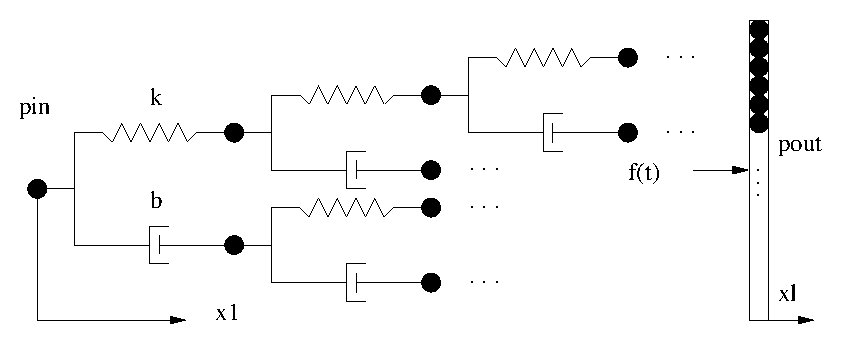
\includegraphics[width=3in]{figs/structure}
    \caption{Infinite tree of springs and dampers.}
    \label{fig:structure}
  \end{figure}
\end{example}

It turns out that if we consider the network to be infinitely large, \textit{i.e.}, an infinite number of bifurcating generations, it is easier to determine the transfer function describing we want, which is
\begin{equation}
  G(s) = \frac{X_{last}(s) - X_1(s)}{F(s)}
  \label{eq:xfer}
\end{equation}
and which describes the relationship between the applied force and deflection of the network. The reason it is easier, is that the network is \emph{self-similar}. If there are an infinite number of generations, if we look at any specific node, then the transfer function from that node to the right end, is the same as any other node to the right end. In other words, from any node, there is an infinite tree growing to the right. 

As such, the transfer function from the first node to the end, is equal to the transfer function from one of the nodes in the second generation to the end, as is illustrated in Figure~\ref{fig:selfsimilar}.

\begin{figure}
  \centering
  \psfrag{k}{$k$}
  \psfrag{b}{$b$}
  \psfrag{pin}{$p_{in}$}
  \psfrag{pout}{$p_{out}$}
  \psfrag{x1}{$x_1$}
  \psfrag{xl}{$x_{last}$}
  \psfrag{f(t)}{$f(t)$}
  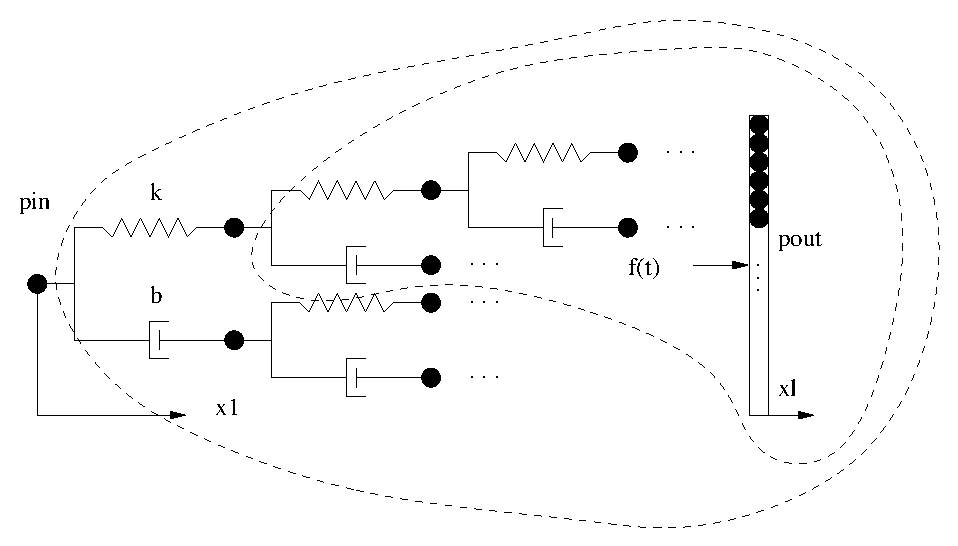
\includegraphics[width=3in]{figs/structure3}
  \caption{Self-similar network where the transfer function from the beginning to end of each outlined region must be equal.}
  \label{fig:selfsimilar}
\end{figure}

Let $G_\infty(s)$ represent the infinite transfer function from any node to the end, and let the transfer function corresponding to the individual components be
\begin{equation}
  G_1(s) = \frac{1}{k} \qquad G_2(s) = \frac{1}{bs}.
  \label{eq:selfsimilarbuild}
\end{equation}

If there are an infinite number of generations then
\[
  G_\infty(s) = \frac{1}{\frac{1}{G_1(s) + G_\infty(s)} +
  \frac{1}{G_2(s) + G_\infty(s)}},
\]
and solving this for $G_\infty(s)$ gives
\[
  G_\infty(s) = \sqrt{G_1(s) G_2(s)} =\sqrt{\frac{1}{k b s }} = \frac{1}{\sqrt{kb}} \frac{1}{\sqrt{s}}.
\] 
where the $G_\infty(s)$ on the left hand side is the transfer function for the entire network, and the two $G_\infty(s)$ terms in the denominator are the transfer functions from the two nodes in the second generation to the end. So this system should be characterized by half-order dynamics because $\sqrt{s} = s^{1/2}$.

\begin{figure}
  \centering
  % GNUPLOT: LaTeX picture with Postscript
\begingroup
  \makeatletter
  \providecommand\color[2][]{%
    \GenericError{(gnuplot) \space\space\space\@spaces}{%
      Package color not loaded in conjunction with
      terminal option `colourtext'%
    }{See the gnuplot documentation for explanation.%
    }{Either use 'blacktext' in gnuplot or load the package
      color.sty in LaTeX.}%
    \renewcommand\color[2][]{}%
  }%
  \providecommand\includegraphics[2][]{%
    \GenericError{(gnuplot) \space\space\space\@spaces}{%
      Package graphicx or graphics not loaded%
    }{See the gnuplot documentation for explanation.%
    }{The gnuplot epslatex terminal needs graphicx.sty or graphics.sty.}%
    \renewcommand\includegraphics[2][]{}%
  }%
  \providecommand\rotatebox[2]{#2}%
  \@ifundefined{ifGPcolor}{%
    \newif\ifGPcolor
    \GPcolorfalse
  }{}%
  \@ifundefined{ifGPblacktext}{%
    \newif\ifGPblacktext
    \GPblacktexttrue
  }{}%
  % define a \g@addto@macro without @ in the name:
  \let\gplgaddtomacro\g@addto@macro
  % define empty templates for all commands taking text:
  \gdef\gplbacktext{}%
  \gdef\gplfronttext{}%
  \makeatother
  \ifGPblacktext
    % no textcolor at all
    \def\colorrgb#1{}%
    \def\colorgray#1{}%
  \else
    % gray or color?
    \ifGPcolor
      \def\colorrgb#1{\color[rgb]{#1}}%
      \def\colorgray#1{\color[gray]{#1}}%
      \expandafter\def\csname LTw\endcsname{\color{white}}%
      \expandafter\def\csname LTb\endcsname{\color{black}}%
      \expandafter\def\csname LTa\endcsname{\color{black}}%
      \expandafter\def\csname LT0\endcsname{\color[rgb]{1,0,0}}%
      \expandafter\def\csname LT1\endcsname{\color[rgb]{0,1,0}}%
      \expandafter\def\csname LT2\endcsname{\color[rgb]{0,0,1}}%
      \expandafter\def\csname LT3\endcsname{\color[rgb]{1,0,1}}%
      \expandafter\def\csname LT4\endcsname{\color[rgb]{0,1,1}}%
      \expandafter\def\csname LT5\endcsname{\color[rgb]{1,1,0}}%
      \expandafter\def\csname LT6\endcsname{\color[rgb]{0,0,0}}%
      \expandafter\def\csname LT7\endcsname{\color[rgb]{1,0.3,0}}%
      \expandafter\def\csname LT8\endcsname{\color[rgb]{0.5,0.5,0.5}}%
    \else
      % gray
      \def\colorrgb#1{\color{black}}%
      \def\colorgray#1{\color[gray]{#1}}%
      \expandafter\def\csname LTw\endcsname{\color{white}}%
      \expandafter\def\csname LTb\endcsname{\color{black}}%
      \expandafter\def\csname LTa\endcsname{\color{black}}%
      \expandafter\def\csname LT0\endcsname{\color{black}}%
      \expandafter\def\csname LT1\endcsname{\color{black}}%
      \expandafter\def\csname LT2\endcsname{\color{black}}%
      \expandafter\def\csname LT3\endcsname{\color{black}}%
      \expandafter\def\csname LT4\endcsname{\color{black}}%
      \expandafter\def\csname LT5\endcsname{\color{black}}%
      \expandafter\def\csname LT6\endcsname{\color{black}}%
      \expandafter\def\csname LT7\endcsname{\color{black}}%
      \expandafter\def\csname LT8\endcsname{\color{black}}%
    \fi
  \fi
  \setlength{\unitlength}{0.0500bp}%
  \begin{picture}(3938.00,2756.00)%
    \gplgaddtomacro\gplbacktext{%
      \colorrgb{0.00,0.00,0.00}%
      \put(391,1637){\makebox(0,0)[r]{\strut{}-30}}%
      \colorrgb{0.00,0.00,0.00}%
      \put(391,1822){\makebox(0,0)[r]{\strut{}-20}}%
      \colorrgb{0.00,0.00,0.00}%
      \put(391,2007){\makebox(0,0)[r]{\strut{}-10}}%
      \colorrgb{0.00,0.00,0.00}%
      \put(391,2192){\makebox(0,0)[r]{\strut{}0}}%
      \colorrgb{0.00,0.00,0.00}%
      \put(391,2378){\makebox(0,0)[r]{\strut{}10}}%
      \colorrgb{0.00,0.00,0.00}%
      \put(511,1409){\makebox(0,0){\strut{}$10^{-4}$}}%
      \colorrgb{0.00,0.00,0.00}%
      \put(1019,1409){\makebox(0,0){\strut{}$10^{-3}$}}%
      \colorrgb{0.00,0.00,0.00}%
      \put(1528,1409){\makebox(0,0){\strut{}$10^{-2}$}}%
      \colorrgb{0.00,0.00,0.00}%
      \put(2036,1409){\makebox(0,0){\strut{}$10^{-1}$}}%
      \colorrgb{0.00,0.00,0.00}%
      \put(2545,1409){\makebox(0,0){\strut{}$10^{0}$}}%
      \colorrgb{0.00,0.00,0.00}%
      \put(3054,1409){\makebox(0,0){\strut{}$10^{1}$}}%
      \colorrgb{0.00,0.00,0.00}%
      \put(3562,1409){\makebox(0,0){\strut{}$10^{2}$}}%
      \colorrgb{0.00,0.00,0.00}%
      \put(-189,2078){\rotatebox{90}{\makebox(0,0){\strut{}$\left| G ( i \omega ) \right| $ [dB]}}}%
    }%
    \gplgaddtomacro\gplfronttext{%
    }%
    \gplgaddtomacro\gplbacktext{%
      \colorrgb{0.00,0.00,0.00}%
      \put(391,390){\makebox(0,0)[r]{\strut{}-80}}%
      \colorrgb{0.00,0.00,0.00}%
      \colorrgb{0.00,0.00,0.00}%
      \put(391,593){\makebox(0,0)[r]{\strut{}-60}}%
      \colorrgb{0.00,0.00,0.00}%
      \colorrgb{0.00,0.00,0.00}%
      \put(391,796){\makebox(0,0)[r]{\strut{}-40}}%
      \colorrgb{0.00,0.00,0.00}%
      \colorrgb{0.00,0.00,0.00}%
      \put(391,999){\makebox(0,0)[r]{\strut{}-20}}%
      \colorrgb{0.00,0.00,0.00}%
      \colorrgb{0.00,0.00,0.00}%
      \put(391,1202){\makebox(0,0)[r]{\strut{}0}}%
      \colorrgb{0.00,0.00,0.00}%
      \put(511,103){\makebox(0,0){\strut{}$10^{-4}$}}%
      \colorrgb{0.00,0.00,0.00}%
      \put(1019,103){\makebox(0,0){\strut{}$10^{-3}$}}%
      \colorrgb{0.00,0.00,0.00}%
      \put(1528,103){\makebox(0,0){\strut{}$10^{-2}$}}%
      \colorrgb{0.00,0.00,0.00}%
      \put(2036,103){\makebox(0,0){\strut{}$10^{-1}$}}%
      \colorrgb{0.00,0.00,0.00}%
      \put(2545,103){\makebox(0,0){\strut{}$10^{0}$}}%
      \colorrgb{0.00,0.00,0.00}%
      \put(3054,103){\makebox(0,0){\strut{}$10^{1}$}}%
      \colorrgb{0.00,0.00,0.00}%
      \put(3562,103){\makebox(0,0){\strut{}$10^{2}$}}%
      \colorrgb{0.00,0.00,0.00}%
      \put(-189,772){\rotatebox{90}{\makebox(0,0){\strut{}$\angle G (i \omega ) $ [deg]}}}%
      \colorrgb{0.00,0.00,0.00}%
      \put(2036,-197){\makebox(0,0){\strut{}Frequency [rad/s]}}%
    }%
    \gplgaddtomacro\gplfronttext{%
    }%
    \gplbacktext
    \put(0,0){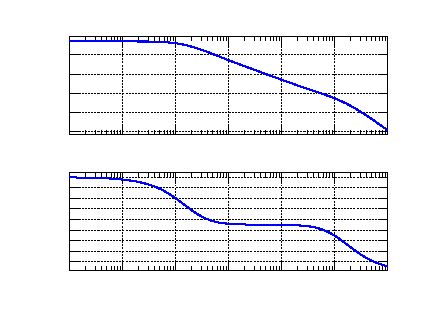
\includegraphics{figs/bodeelement}}%
    \gplfronttext
  \end{picture}%
\endgroup

  \caption{Network stress-strain frequency response.}
  \label{fig:bodeelement}
\end{figure}

Consistent with the idea above about fractional order systems ``converging'' to integer order ones, we plot the Bode plot for a network of this type where there are five generations with $k =1$ and The Bode plot for this system is illustrated in Figure~\ref{fig:bodeelement}, which is characterized by two half-order dynamics features. First, the slope of the high frequency portion of the magnitude plot is $-10$dB/decade and the phase is $-45^\circ$. Because first order terms are characterized by a slope of $-20$dB/decade and a phase of $-90^\circ$, these features make sense as half order effects.

\subsection{Ultrasound Example}
Reference and summaries Holm's paper.

